% \begin{frame}
%     - was ist tailcuts?
%     - wo liegt der unterschied? -> besonders zeitkomponente
%     - ist die schon richtig drin in cta?
%     - cleaning level von tailcuts ableiten
%     - vergleich auf schauerbildern
%     - extremfälle: was bringt das?
%     - Effekt auf ML
% \end{frame}

\section{Alternative cleaning method}
\begin{frame}{Cleaning methods}
    \begin{columns}[T] % align columns
        \begin{column}{.48\textwidth}
            Tailcuts Cleaning
            \begin{enumerate}
                \item "two treshold procedure"
                \item pixels above t1 will be kept
                \item neighboring pixels above t2 will be kept
                \item "lonely" pixels wont survive
            \end{enumerate}
        \end{column}
        \begin{column}{.48\textwidth}
            FACT image cleaning
            \begin{enumerate}
                \item similar behaviour, but also uses information about the arrival times
                \item pixels with a very different arrival time than their neighbours get removed
                %\item for now arrival times are integers in ctapipe -> limits search for optimal threshold
                \item removes "lonely" pixels multiple times
                \item one would assume less separated pixels
                \item intensity threshold should probably be a bit more loose than with tailcuts
        \end{enumerate}
        \end{column}
    \end{columns}
\end{frame}

\begin{frame}{timing information}
    \begin{figure}
        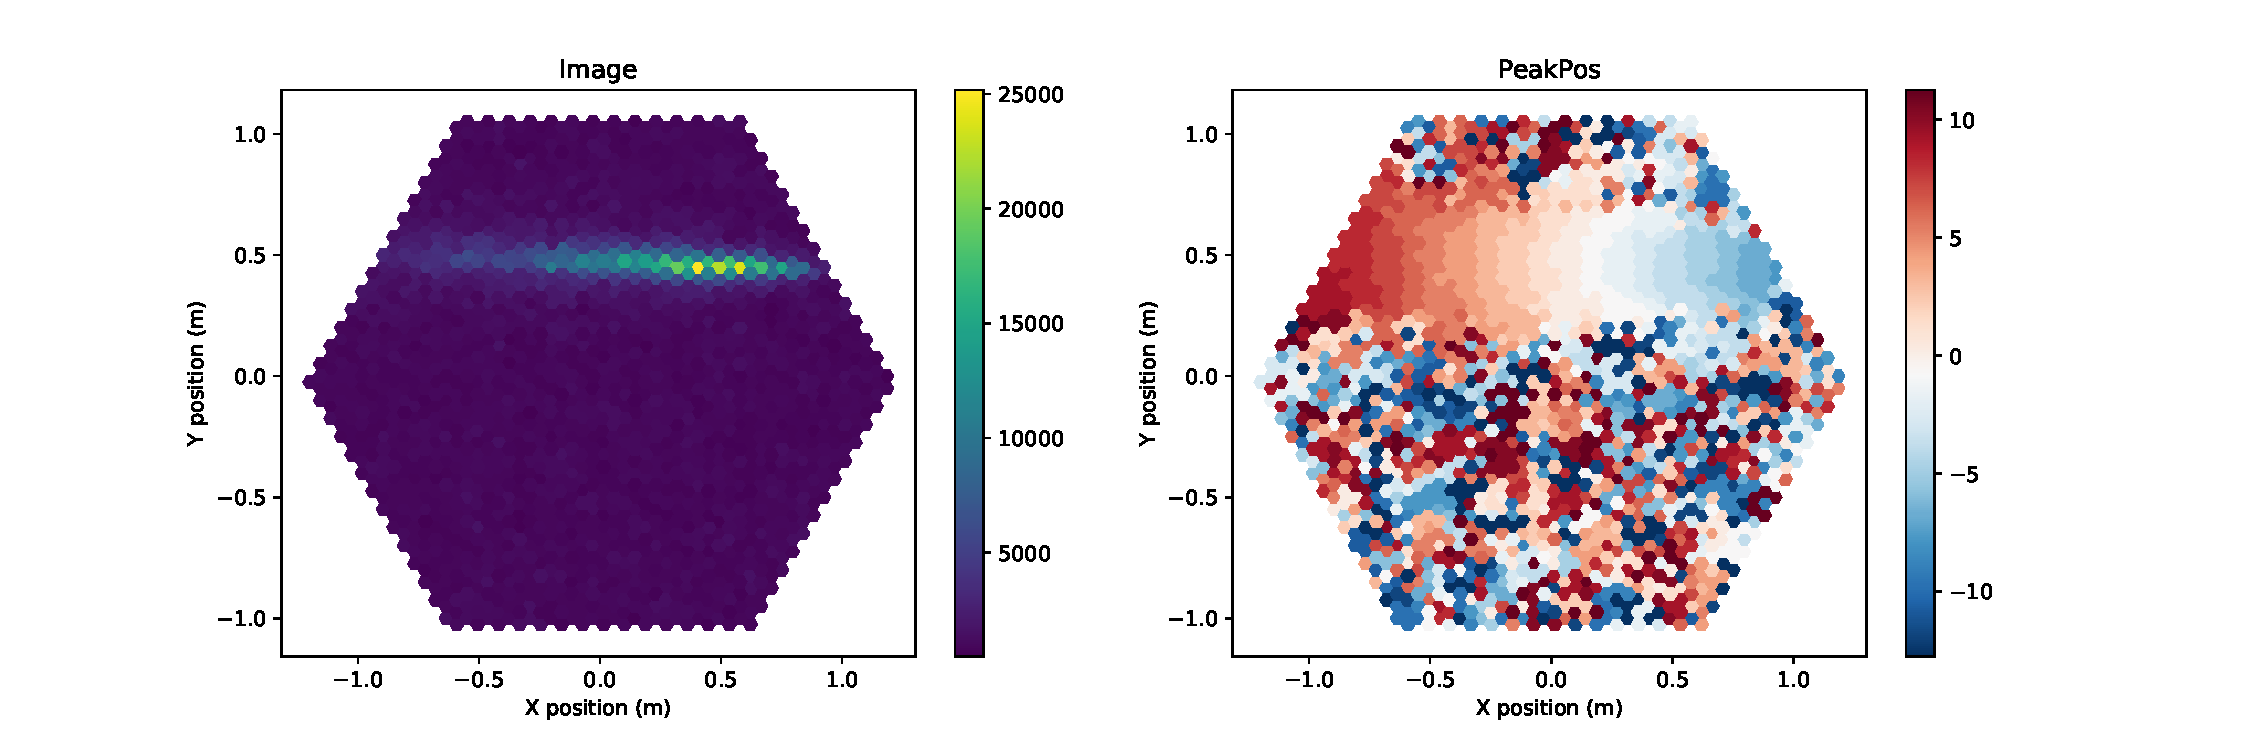
\includegraphics[width=\linewidth]{images/peakpos.pdf}
    \end{figure}
    Intensity and relative arrival time for a MC gamma-event
\end{frame}

